\section{Euler方法}
\label{sec:odenum-euler}

式~\eqref{eq:odenum-integral-step}的积分里，被积函数在这一步内部未知。最朴素的办法是假装它在这一步内不变，取起点的值。这样得到的方法是什么样，一步偏差多大，走完整个区间又要算多少次？

\paragraph{主要思想}
方向场在每个点$(t,\bm{x})$上给出一个速度$\bm{f}(t,\bm{x})$。站在当前点，读一次速度，沿这个方向走$h$的时间，到达新位置后再读一次，这就是\term{显式Euler方法}（explicit Euler method）。它像顺水漂流时每隔一段时间才看一眼水流方向：两次观察之间，方向按上一次的读数保持不变。类比的界限在于：真实的漂流者一直被水流带动，折线在两次读数之间却完全不看水流。

积分的说法与此相同。用$\bm{f}(t_k,\bm{x}^{(k)})$代替式~\eqref{eq:odenum-integral-step}中的被积函数，积分变成长度$h$乘以这个常向量，得到
\begin{equation}
 \bm{x}^{(k+1)}=\bm{x}^{(k)}+h\,\bm{f}\bigl(t_k,\bm{x}^{(k)}\bigr).
 \label{eq:odenum-euler}
\end{equation}

“显式”是指新值已经写在等号左边，右端只用旧值，代入即得。图~\ref{fig:odenum-euler-polygon}是这样得到的折线：每段都沿所在点的方向场切出去。真解沿方向场连续弯曲，折线每走一段才改一次方向，所以总是落在真解的一侧或另一侧。步长缩小后，改方向更频繁，折线更贴近真解。

\begin{BookInlineFigure}
 \centering
 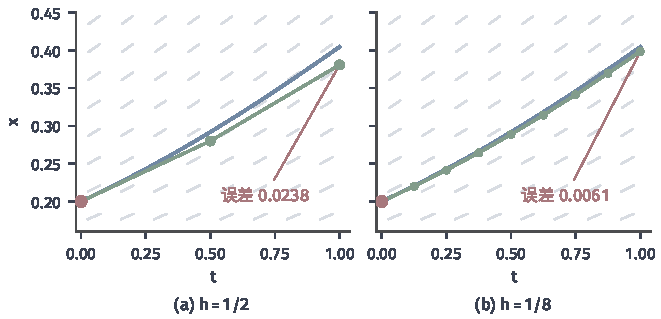
\includegraphics[width=112mm]{figures/06-differential-equations/01-ordinary-differential-equations/matplotlib/odenum-euler-polygon/figure.pdf}
 \caption{显式Euler折线与方向场。灰色短线是$\dot{x}=x(1-x)$的方向场，蓝线为$x(0)=0.2$的真解，绿线和绿点为数值解。(a)$h=1/2$；(b)$h=1/8$。红色标注是$t=1$处的绝对误差。}
 \label{fig:odenum-euler-polygon}
\end{BookInlineFigure}

\paragraph{计算过程}
下面用贯穿全章的初值问题逐步演示，数据为
\begin{equation}
 \dot{x}=x(1-x),\qquad x(0)=0.2,\qquad T=1.
 \label{eq:odenum-running}
\end{equation}
分离变量可得真解，它用来核对数值结果：
\begin{equation}
 x(t)=\frac{1}{1+4\mathrm{e}^{-t}}.
 \label{eq:odenum-running-exact}
\end{equation}
取$h=1/2$，于是$N=2$，手算两步即可走完。

\needspace{6\baselineskip}
\paragraph{变量}
\begin{itemize}
 \item $\bm{x}^{(k)}\in\mathbb{R}^{n}$：第$k$个网格点的数值解。
 \item $t_k$：当前时刻。
 \item $\bm{s}^{(k)}\in\mathbb{R}^{n}$：当前点读到的斜率。
\end{itemize}

\paragraph{初始化}
把数值解初始化为初值，时刻初始化为起点，步长和步数由区间决定：
\[
 \bm{x}^{(0)}=\bm{x}_0,\qquad t_0\text{给定},\qquad h=T/N.
\]
例中
\[
 x^{(0)}=0.2,\qquad t_0=0,\qquad h=0.5,\qquad N=2.
\]

\needspace{6\baselineskip}
\paragraph{每轮更新}
对$k=0,1,\ldots,N-1$依次执行：
\begin{enumerate}
 \item \textbf{读取斜率。}计算
 \[
  \bm{s}^{(k)}=\bm{f}\bigl(t_k,\bm{x}^{(k)}\bigr).
 \]
 例中第一轮
 \[
  s^{(0)}=0.2\times(1-0.2)=0.16.
 \]
 \item \textbf{沿斜率走一步。}由式~\eqref{eq:odenum-euler}计算
 \[
  \bm{x}^{(k+1)}=\bm{x}^{(k)}+h\,\bm{s}^{(k)},\qquad t_{k+1}=t_k+h.
 \]
 例中第一轮
 \[
  x^{(1)}=0.2+0.5\times0.16=0.28,\qquad t_1=0.5.
 \]
 例中第二轮先读斜率，再走一步：
 \[
  s^{(1)}=0.28\times0.72=0.2016,\qquad x^{(2)}=0.28+0.5\times0.2016=0.3808.
 \]
 \item \textbf{停止。}当$k+1=N$时结束。例中$k+1=2$，退出循环。
\end{enumerate}
最终得到网格值$\bm{x}^{(0)},\ldots,\bm{x}^{(N)}$。例中$x^{(2)}=0.3808$，而由式~\eqref{eq:odenum-running-exact}，$x(1)\approx0.404610$，误差约为$-0.0238$。

\paragraph{局部误差}
偏差从何而来？按定义~\ref{def:odenum-errors}，把真解代入一步更新。设$\bm{x}(t)$二次连续可微，含积分余项的Taylor公式给出
\[
 \bm{x}(t_{k+1})=\bm{x}(t_k)+h\dot{\bm{x}}(t_k)+\int_{t_k}^{t_{k+1}}(t_{k+1}-s)\ddot{\bm{x}}(s)\,\mathrm{d}s.
\]
真解满足$\dot{\bm{x}}(t_k)=\bm{f}(t_k,\bm{x}(t_k))$，这一项正好是Euler方法走的那一步，相减后只剩余项。于是显式Euler方法的局部截断误差是
\begin{equation}
 \bm{\ell}^{(k+1)}=-\int_{t_k}^{t_{k+1}}(t_{k+1}-s)\ddot{\bm{x}}(s)\,\mathrm{d}s.
 \label{eq:odenum-euler-local}
\end{equation}
权函数$t_{k+1}-s$在这一步上的积分是$h^2/2$，取范数得到局部误差界
\begin{equation}
 \bigl\lVert\bm{\ell}^{(k+1)}\bigr\rVert_2\leq\frac{h^2}{2}\max_{t\in[t_0,t_0+T]}\bigl\lVert\ddot{\bm{x}}(t)\bigr\rVert_2.
 \label{eq:odenum-euler-local-bound}
\end{equation}

$\ddot{\bm{x}}$由方程自身决定。若$\bm{f}$连续可微，对$\dot{\bm{x}}=\bm{f}(t,\bm{x})$用链式法则，得到
\[
 \ddot{\bm{x}}=\partial_t\bm{f}+\partial_{\bm{x}}\bm{f}\,\bm{f},
\]
右端在$(t,\bm{x}(t))$处取值。$\ddot{\bm{x}}$衡量解曲线弯得多厉害，弯得越厉害，直线走一步偏得越远。

在例~\eqref{eq:odenum-running}中，$\bm{f}$不显含时间，且$\ddot{x}=(1-2x)\dot{x}$。在$t=0$处
\[
 \ddot{x}(0)=(1-0.4)\times0.16=0.096,
\]
所以第一步局部误差的主要部分是$-0.048h^2$。$h=1/2$时它等于$-0.012$，实际的第一步误差是$0.28-0.291875=-0.011875$，两者很接近。图~\ref{fig:odenum-euler-one-step}左侧画出这段偏差，右侧显示步长减半时偏差变为约四分之一。

\begin{BookInlineFigure}
 \centering
 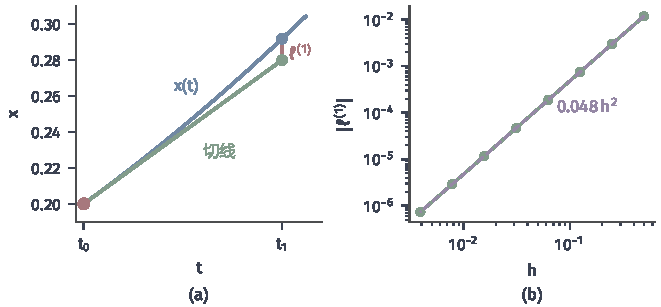
\includegraphics[width=112mm]{figures/06-differential-equations/01-ordinary-differential-equations/matplotlib/odenum-euler-one-step/figure.pdf}
 \caption{显式Euler方法的第一步。(a)$h=1/2$：蓝线是真解，绿线是起点处的切线，红色线段是局部截断误差$\ell^{(1)}$。(b)绿点是不同步长下的$\lvert\ell^{(1)}\rvert$，紫色虚线是主要部分$0.048h^2$。}
 \label{fig:odenum-euler-one-step}
\end{BookInlineFigure}

\begin{definition}[方法的阶]
 \label{def:odenum-order}
 设一步方法的局部截断误差沿真解满足：存在与$k$、$h$无关的$C$和$h_0>0$，使当$0<h\leq h_0$时，对所有$k$有
 \begin{equation}
  \bigl\lVert\bm{\ell}^{(k+1)}\bigr\rVert_2\leq Ch^{p+1},
  \label{eq:odenum-order}
 \end{equation}
 就称方法在这个问题上具有\term{局部误差阶}（local order）$p+1$，称$p$为\term{方法的阶}（order of a method）。
\end{definition}

由式~\eqref{eq:odenum-euler-local-bound}，当$\bm{x}\in C^2$时显式Euler方法的阶为$1$。一步误差$h^2$，方法的阶却是$1$，原因是走完$T$要$N=T/h$步，$N\cdot h^2$恰好是$Th$。这个数步数的算术还不是证明，第~\ref{sec:odenum-error-convergence}节将补全它需要的条件。

\paragraph{步长细化的比较}
一个基本的检验是把步长不断减半，看终点误差怎样变化。表~\ref{tab:odenum-euler-refine}列出例~\eqref{eq:odenum-running}的结果。显式Euler方法每步求值一次右端，所以$N$同时就是计算量。

\begin{BookInlineTable}
 \centering
 \caption{显式Euler方法的步长细化。问题为式~\eqref{eq:odenum-running}，误差指$x^{(N)}-x(1)$，比值是上一行误差除以本行误差。}
 \label{tab:odenum-euler-refine}
 \begin{tabular}{rrrrr}
  \toprule
  $N$ & $h$ & $x^{(N)}$ & 误差 & 比值\\
  \midrule
  2 & 0.5 & 0.380800 & $-2.381\times10^{-2}$ & \\
  4 & 0.25 & 0.392434 & $-1.218\times10^{-2}$ & 1.95\\
  8 & 0.125 & 0.398476 & $-6.134\times10^{-3}$ & 1.99\\
  16 & 0.0625 & 0.401535 & $-3.075\times10^{-3}$ & 1.99\\
  32 & 0.03125 & 0.403071 & $-1.539\times10^{-3}$ & 2.00\\
  \bottomrule
 \end{tabular}
\end{BookInlineTable}

比值趋于$2$：计算量加倍，误差只减半。把误差写成$0.0493/N$（图~\ref{fig:odenum-euler-refinement}），可知要把误差压到$10^{-6}$，约需$5\times10^{4}$次右端求值。对这样一个简单方程，这个价钱是昂贵的，它也给后面的高阶方法提供了比较的基准。

\begin{BookInlineFigure}
 \centering
 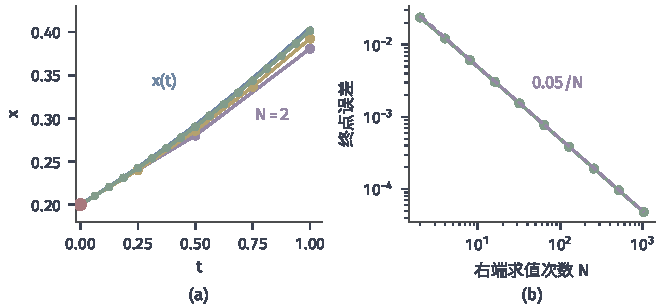
\includegraphics[width=112mm]{figures/06-differential-equations/01-ordinary-differential-equations/matplotlib/odenum-euler-refinement/figure.pdf}
 \caption{显式Euler方法的步长细化。(a)蓝线是真解，紫、黄、绿折线分别是$N=2,4,16$的数值解。(b)$t=1$处的误差随右端求值次数$N$的变化，紫色虚线是参考直线$0.05/N$。}
 \label{fig:odenum-euler-refinement}
\end{BookInlineFigure}

